\begin{frame}[standout]

    Bases de données orientées colonne

\end{frame}

\begin{frame}{Caractéristiques des bases de données orientées colonne}

    \begin{definitionbox}
        Dans une base de données orientée colonne, les données sont stockées par \textbf{colonnes} plutôt que par lignes.

        Chaque ligne correspond à une clé unique, et les colonnes stockent des paires de \textbf{nom-colonne : valeur}, ce qui permet de regrouper des colonnes similaires pour une meilleure performance des requêtes en lecture.
    \end{definitionbox}

    \begin{noteblock}
        \begin{itemize}
            \item Optimisé pour les lectures massives sur des colonnes spécifiques.
            \item Très scalable et performant pour des requêtes analytiques.
        \end{itemize}
        $\hookrightarrow$ Idéal pour des applications nécessitant des analyses de grandes quantités de données.
    \end{noteblock}
\end{frame}

\begin{frame}{Bases de données orientées colonne}
    \begin{figure}[htb]
        \centering
        \begin{tikzpicture}
            \node[minimum width=3cm, minimum height=2cm] at (0, 0) {\includesvg[height=1.1cm]{img/db/cassandra.svg}};
            \node[minimum width=3cm, minimum height=2cm] at (4, 0) {\includesvg[height=0.9cm]{img/db/hbase.svg}};
            \node[minimum width=3cm, minimum height=2cm] at (0, -2) {\includesvg[height=0.7cm]{img/db/druid.svg}};
            \node[minimum width=3cm, minimum height=2cm] at (4, -2) {
\includegraphics[height=1.5cm]{img/db/scylla-db.png}};
            \node[minimum width=3cm, minimum height=2cm] at (0, -4) {
\includegraphics[height=1cm]{img/db/gcp-bigtable.png}};
            \node[minimum width=3cm, minimum height=2cm] at (4, -4) {
\includegraphics[height=1cm]{img/db/hypertable.png}};
        \end{tikzpicture}
    \end{figure}
\end{frame}

\begin{frame}{Exemple : distribution des données sur Cassandra}

    \begin{figure}
        \centering
        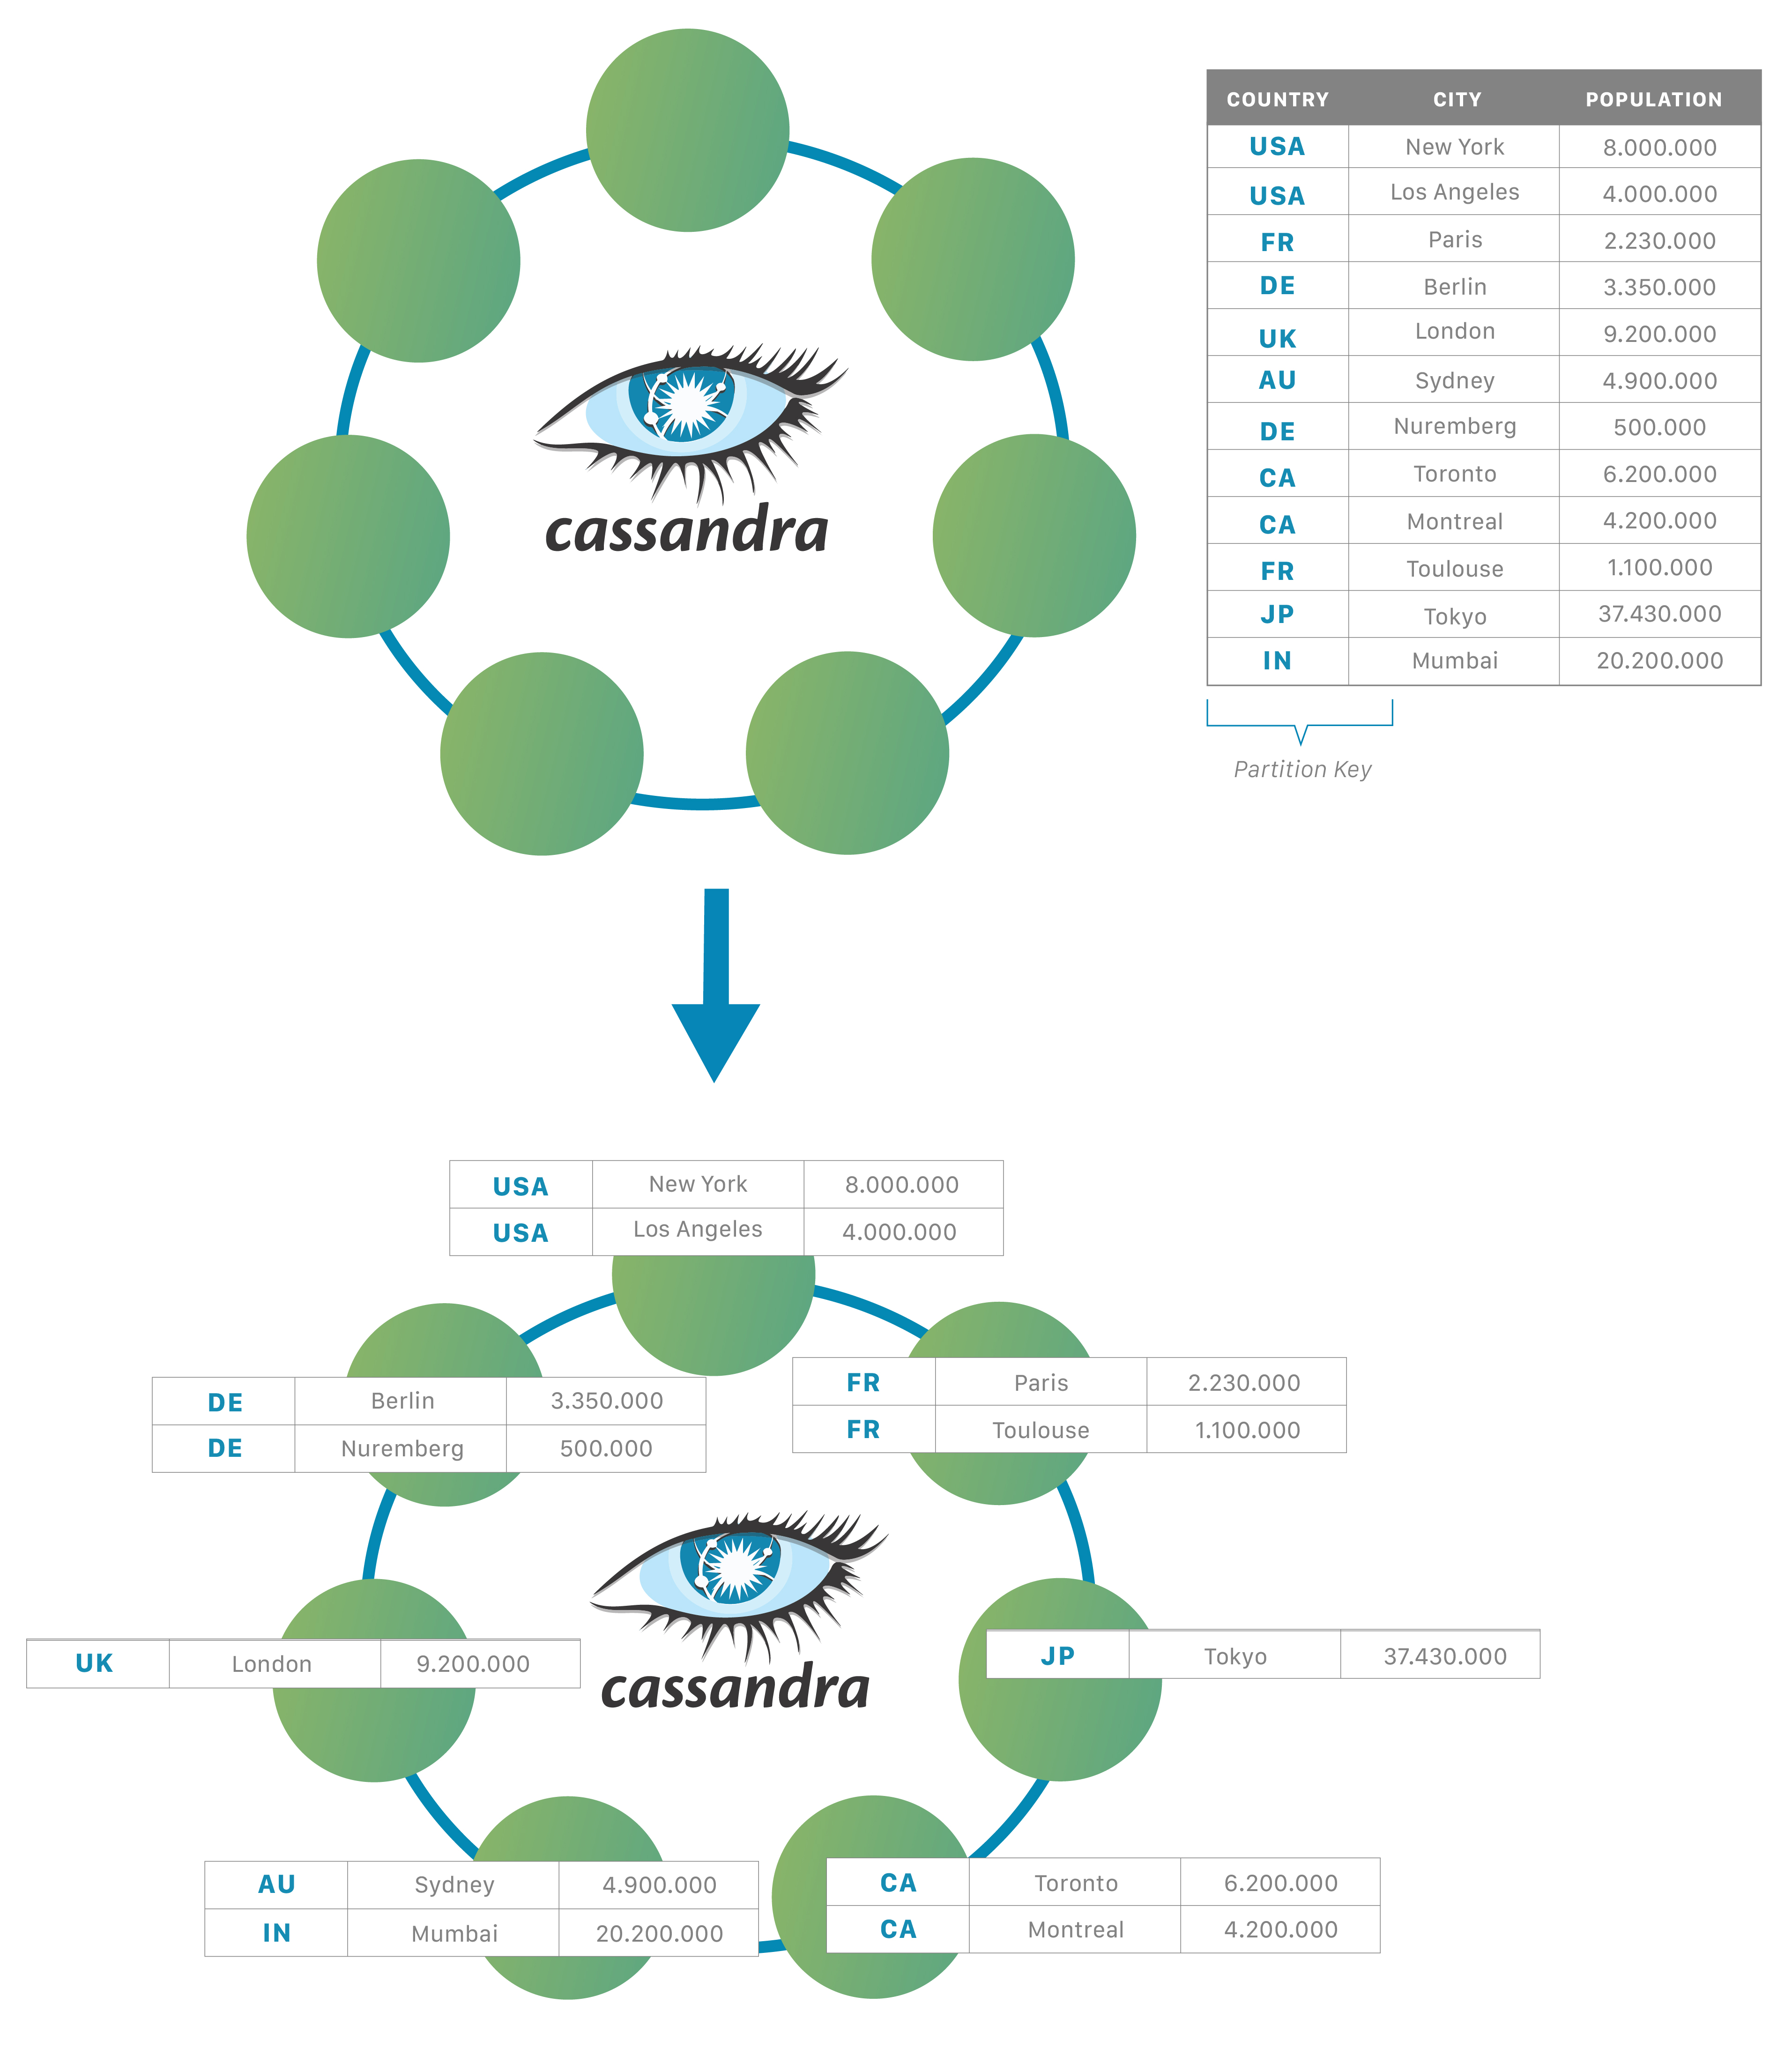
\includegraphics[width=0.8\textheight]{img/apache-cassandra-nodes.jpg}
    \end{figure}

\end{frame}

\begin{frame}{Cas d'usages des bases de données orientées colonne}

\begin{itemize}
    \item \textbf{Systèmes de gestion des données financières}\\
    $\hookrightarrow$ Permet d'extraire rapidement des colonnes spécifiques comme les prix ou les transactions sur de grands ensembles de données.
    \vspace{0.3cm}

    \item \textbf{Outils analytiques et de Big Data}\\
    $\hookrightarrow$ Optimisé pour les requêtes analytiques complexes sur des jeux de données massifs.
    \vspace{0.3cm}

    \item \textbf{Moteurs de recommandation}\\
    $\hookrightarrow$ Stocke des informations sur les utilisateurs et leurs préférences sous forme de colonnes, permettant une extraction rapide pour les recommandations en temps réel.
\end{itemize}
\end{frame}

\begin{frame}{Avantages et inconvénients des bases de données colonne}
\vfill
\prosbox{
    \textbf{Avantages}
    \begin{itemize}
        \item Très performant pour les requêtes en lecture sur des colonnes spécifiques.
        \item Scalabilité horizontale adaptée pour le traitement de données massives.
        \item Idéal pour des applications analytiques ou des systèmes OLAP.
    \end{itemize}
}
\vfill
\pause
\consbox{
    \textbf{Inconvénients}
    \begin{itemize}
        \item Moins efficace pour des écritures fréquentes ou des transactions complexes.
        \item Complexité accrue pour gérer les relations entre colonnes.
    \end{itemize}
}
\vfill
\end{frame}

\begin{frame}{Focus sur Apache Cassandra}

\end{frame}

\begin{frame}{Étude de cas}

    Netflix et Cassandra (scalabilité pour le streaming).

    Problématique.
    Solution NoSQL choisie.
    Architecture mise en place.
    Résultats (performances, coûts).

\end{frame}
